Obiettivo del controllo orbitale è la cancellazione delle forze non
gravitazionali agenti sul satellite per rendere il moto del centro di massa del
satellite dovuto con accettabile approssimazione esclusivamente alle forze
gravitazionali, l'architettura prescelta per la compensazione di queste forze è
basata sull' embedded model i cui concetti fondamentali sono:
\begin{description}
\item[Dinamica Controllabile:] Descrivono la dinamica tra comando e misura, deve
catturare le dinamiche ad alta frequenza il più vicino possibile alla più alta
componente in frequenza dei disturbi da cancellare.
\item[Dinamica del Disturbo:] Dinamica rappresentante il disturbo e modellata su
base statistica.
\end{description} 

\begin{figure}
\includegraphics[page=13, trim=2.5cm 18.5cm 3cm 3cm,
clip=true,width=\textwidth]{control/orbit_control/images/cap7.pdf}
\caption{Control architecture}
\end{figure}